\chapter{A Top down view of the architecture}
\label{architecure}
Every Digital System is always divided in two big blocks, as it can be also observed in Figure \ref{fig:dlxarch}:
\begin{itemize}
\item Control Unit, it is the brain of the processor and it is in charge of handling the synchronization between stages asserting the proper signals.
\item Datapath, it is the actual brawn of the processor. It is composed by 5 functional units (meaning that it is a 5 stage pipeline processor) that perform data processing operations on data.
\end{itemize}

\begin{figure}[!htbp]
\centering
\captionsetup{justification=centering}
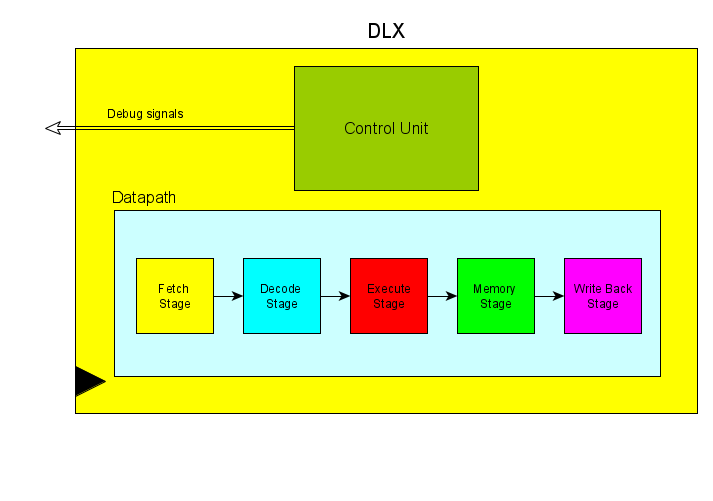
\includegraphics[scale=0.5,angle=0]{./chapters/figures/dlx_top.png}
\caption{DLX top level entity}
\label{fig:dlxarch}
\end{figure}

Notice that the clock and reset signal are routed to every unit (interconnections missing in Figure \ref{fig:dlxarch} for increasing readability). Moreover, the debug signals are present only for simulation purposes, they are removed during the synthesis by means of synthesis pragma.

\newpage
\section{Control Unit}
The brain of the processor is a simple control unit based on two states, fetch and decode. However, the fetch state is executed only at the reset, leading to have a nop operation in the pipeline operation. Meanwhile, when the processor is fully operational, it is always in decode state.\\\\
The control unit is based on the hardwired approach, meaning that for each one of the instruction there is a predefined signature for signals to be asserted (except for particular case, such as the sub instruction, where the carry in must be set to 1 since the adder is shared among the addition and subtraction). All the predefined signals for given instruction are activated only once. Therefore, for correctly synchronizing the pipeline they have to be properly delayed by mean of registers.\\
The control unit is also in charge of selecting the proper operation for the ALU. During the execution of the integer multiplication, it stalls the pipeline for the whole duration of the operation in order to avoid hazards or it may restore the pipeline behavior in the case that one of the multiplication operands is zero and/or it is bigger than $2^{16}-1$, since the multiplication is between 16-bitwidth operands.

\section{Datapath}
The datapath of the DLX is composed by 5 stages, as in Figure \ref{fig:dp}:
\begin{figure}[!htbp]
\centering
\captionsetup{justification=centering}

\includegraphics[scale=0.35,angle=0]{./chapters/figures/datapath.png}
\caption{Datapath \protect\footnotemark[1] \protect\footnotemark[2]}
\label{fig:dp}
\end{figure}
\footnotetext[1]{Control Unit signals are missing for increasing readability}
\footnotetext[2]{IRAM and DRAM are only logically represented in the pipeline, in reality they are outside the core.}
\newpage
\begin{itemize}
\item Fetch Stage: it uses as address for instruction memory the value of the PC, while the data(instruction) coming from the memory are saved into the IR. It also computes the new value of the PC, a plus 4 during normal operation, and a loop back of the PC value in the case the pipeline is in stall.
\item Decode Stage: it decodes the instruction and depending on the instruction type, it selects the correct values for accessing to the register file and save them in the A and B registers or it extends the value of the immediate field (from 16 bit to 32 bit in case of an immediate instruction or from 26 to 32 bit in case of jump instruction).
\item Execute Stage: The ALU operates on its input, depending on the current operation, and in this stage the condition for taking the branch is eventually evaluated. It is based of an enhanced version of the ALU developed during the laboratories, in which has been added the missing operations of comparison. In addition, the current adder has also been developed during the lab and it is based on the Pentium 4 adder which is shared among the addition and subtraction exploiting the properties of two's complement binary representation.
\item Memory Stage: it is in charge of accessing the memory if needed or load the data from memory in LMD register. It also decides the value of the PC in the case a branch is taken.
\item Write Back Stage: it writes back into the register file either data from ALU or data memory.
\end{itemize}

Moreover, the green registers between each stage (i.e. IF/ID, ID/IE, IE/IM and IM/IWB) are registers used for synchronization purposes of values\footnote{A register preceding or succeeding those unit means that signals inside them are just a wire.}, for example the register index for writing back into the register file need to be delayed by 3 clock cycles (it is needed in the write back stage). Nevertheless, the logical view of Figure \ref{fig:dp}, they are actually implemented in the right stage (if not shown otherwise, such as for the A and B registers).

\subsection{ALU Multiplier}
Another important aspect of the ALU is the integer multiplier.\\
It is based on the Booth's multiplier developed during the lab as in Figure \ref{fig:alumula}.

\begin{figure}[!htbp]
\begin{subfigure}{.5\textwidth}
\centering
% include first image
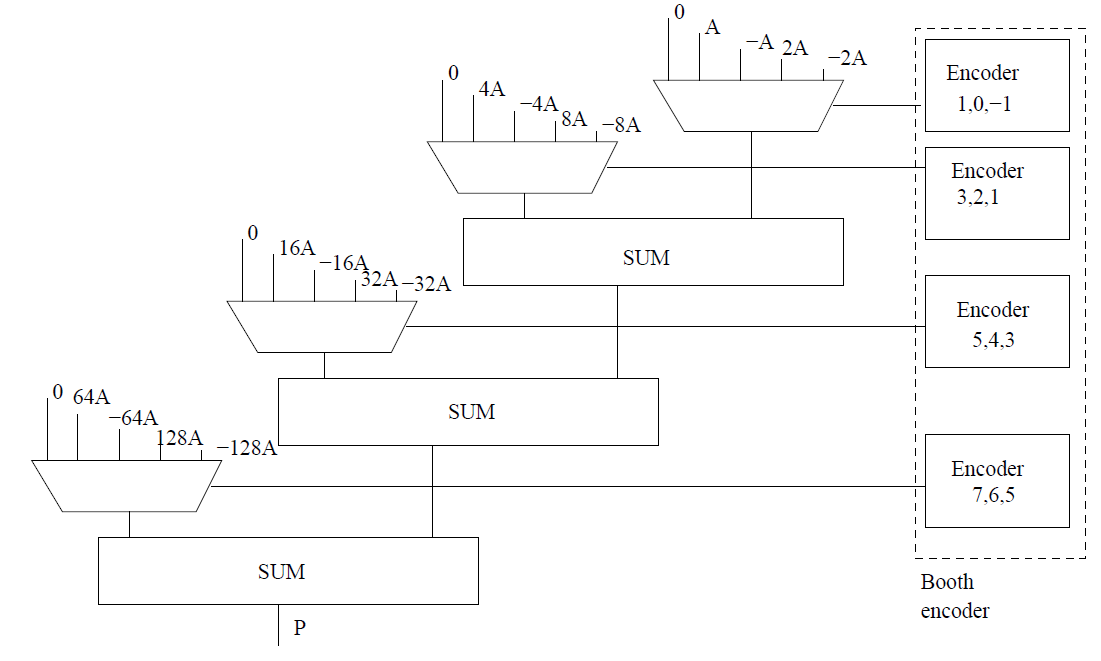
\includegraphics[scale=0.7,width=1\linewidth,height=6cm]{./chapters/figures/mult.PNG}
\caption{Booth's multiplier}
\label{fig:alumula}
\end{subfigure}
\begin{subfigure}{.5\textwidth}
\centering
% include second image
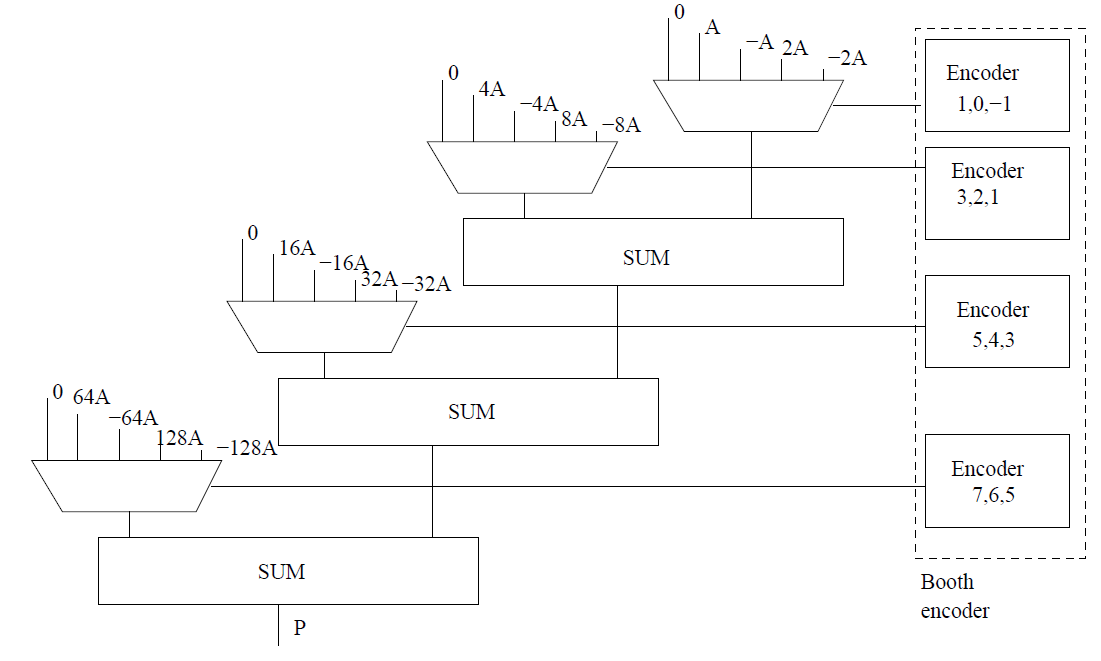
\includegraphics[scale=0.7,width=1\linewidth,height=6cm]{./chapters/figures/mult_pip.PNG}
\caption{Pipelined Booth's multiplier\protect\footnotemark[2]}
\label{fig:alumulb}
\end{subfigure}
\caption{ALU Multiplier}
\label{fig:alumul}
\end{figure}
\footnotetext[2]{Registers are in red}
As it can be seen from Figure \ref{fig:alumulb}\footnote[3]{The Figure represents a 8-bit multiplier. However, the approach is the same, only the internal stages of the multiplier have been pipelined.}, the previously developed unit has been enhanced pipelining it in order to have an 8 stage (6 inside the multiplier and 2 outside the unit, the A and B register and the ALU output register) multiplier, reducing the critical path and increasing the possible achievable performances. It is worth to mention that since the unit is pipeline it can potentially execute in parallel up to 8 multiplication, one after the other without any data hazards and with a proper control unit to handle the specific situation.\\
Moreover, the compiler script has been also modified for adding the integer multiplication and the assigned opcode can be seen in Appendix \ref{appendix8}.